上述算法表明，若对所有 $n$ 都有 $\tilde R_n = \rank(\St_{([n])})$，则存在一个秩为 $(\tilde R_1,\dots, \tilde R_{N-1})$ 的 TT 分解，这说明 $\St$ 的 TT 秩 $(R_1,\dots, R_{N-1})$ 以各矩阵化的秩为上界：对所有 $n$ 有 $ R_n \leq \rank(\St_{([n])} )$。也容易证明 TT 秩以各矩阵化的秩为下界。事实上，设 $\St$ 的 TT 秩为 $(R_1,\dots, R_{N-1})$，则存在一个秩为 $(R_1,\dots, R_{N-1})$ 的 TT 分解。利用定理~\ref{thm: matricization-rank}，容易看出这意味着对所有 $n$ 有 $\rank(\St_{([n])} )\leq  R_n$。
\end{proof}
尽管上面的证明用逐次 QR 分解构造出精确的 TT 分解，但通常被称为 TT-SVD 的算法是对逐次展开施行奇异值分解。在精确情形下，保留全部非零奇异值即得 TT 秩
$
R_n = \rank(\St_{([n])} )
$.
奇异值分解这一形式的优点在于，它直接给出了一个低秩近似算法：在每一步都可使用截断奇异值分解，或截到给定的 TT 秩，或按被舍弃奇异值不超过给定容差来截断~\citep{oseledets2010approximation,holtz2012manifolds}。

另一种被广泛使用的、把张量分解为张量列（tensor train, TT）格式的方法是交替最小二乘（Alternating Least Squares, ALS）算法。在介绍这一方法之前，我们先描述 TT 分解的标准形。
\begin{definition}\label{def:canonical-form}
   若所有 $n<j$ 的核心张量都是左正交的、所有 $n>j$ 的核心张量都是右正交的，则称 TT 分解 $\TT(({\At_n})_{n=1}^N)\in\RR^{d_1\times\dots\times d_N}$ 关于固定指标 $j\in [N]$ 处于标准形；例如，下面的 TT 分解就关于其第三个核心张量处于标准形：
$$
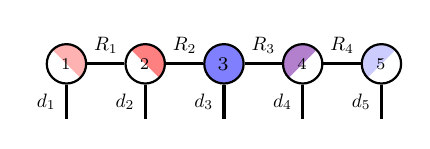
\begin{tikzpicture}[baseline=-0.5ex]
    \tikzset{tensor/.style = {minimum size = 0.5cm,shape = circle,thick,draw=black,inner sep = 0pt}, edge/.style = {thick,line width=.4mm},every loop/.style={}}
    \def\x{0}
    \def\y{0}
 \node[tensor, path picture={
        \fill[fill=red!30!white](path picture bounding box.south east)
        -- 
        (path picture bounding box.north west) --
        (path picture bounding box.north east) -- cycle;
        }, shift={(\x,\y)}] (A) {\scalebox{0.85}{$\At_1$}};
        \draw[edge](A) -- (\x,\y-0.7) node [midway,left] {\scalebox{0.7}{\dimcolor{$d_1$}}};
       \node[tensor, path picture={
        \fill[fill=red!50!white](path picture bounding box.south east)
        -- 
        (path picture bounding box.north west) --
        (path picture bounding box.north east) -- cycle;
        }, shift={(\x+1,\y)}] (B) {\scalebox{0.85}{$\At_2$}};
         \draw[edge](B) -- (\x+1,\y-0.7)node [midway,left] {\scalebox{0.7}{\dimcolor{$d_2$}}};
         \node[tensor,fill=blue!50!white] (C) at (\x+2,\y){$\At_3$};
          \draw[edge](C) -- (\x+2,\y-0.7)node [midway,left] {\scalebox{0.7}{\dimcolor{$d_3$}}};
          \node[tensor, path picture={
        \fill[fill=blue!60!red!50!](path picture bounding box.south west)
        -- 
        (path picture bounding box.north east) --
        (path picture bounding box.north west) -- cycle;
        }, shift={(\x+3,\y)}] (D) {\scalebox{0.85}{$\At_4$}};
         \draw[edge](D) -- (\x+3,\y-0.7)node [midway,left] {\scalebox{0.7}{\dimcolor{$d_4$}}};
           \node[tensor, path picture={
        \fill[fill=blue!20!white](path picture bounding box.south west)
        -- 
        (path picture bounding box.north east) --
        (path picture bounding box.north west) -- cycle;
        }, shift={(\x+4,\y)}] (E) {\scalebox{0.85}{$\At_5$}};
         \draw[edge](E) -- (\x+4,\y-0.7)node [midway,left] {\scalebox{0.7}{\dimcolor{$d_5$}}};
    \draw[edge](A) -- (B) node [midway,above] {\scalebox{0.7}{\dimcolor{$R_1$}}};
    \draw[edge](B) -- (C) node [midway,above] {\scalebox{0.7}{\dimcolor{$R_2$}}};
    \draw[edge](C) -- (D) node [midway,above] {\scalebox{0.7}{\dimcolor{$R_3$}}};
    \draw[edge](D) -- (E) node [midway,above] {\scalebox{0.7}{\dimcolor{$R_4$}}};
\end{tikzpicture}.
$$
$\At_3$ 左侧的核心张量都是左正交的，右侧的核心张量都是右正交的。核心张量 $\At_3$ 称为正交中心。注意，对核心张量施加一系列 QR 分解，就能把任意 TT 分解高效地转化为关于任意指标 $j\in [N]$ 的标准形~\citep{holtz2012alternating,evenbly2018gauge}。
\end{definition}
\paragraph{用交替最小二乘~(ALS) 计算 TT 分解} 单站点张量列交替最小二乘（TT-ALS）方法~\citep{holtz2012alternating} 从一个处于标准形的 TT 分解出发，该分解由一个粗略近似初始化~(例如用随机核心张量，或用 TT-SVD 得到)。
在第一步中，分解的核心张量 
$\At_1$ 是非正交的。在自左向右（相应地，自右向左）的扫描过程中，算法固定除第 $n$ 个核心张量 $\At_n$ 之外的所有核心张量，并对其加以优化，使其与目标张量之间的距离最小。由此得到的极小化问题是一个简单的最小二乘问题，故得名 ALS。  
更新 $\At_n$ 之后，施加一次 QR 分解以保证数值稳定性并维持标准形。非标准正交的因子随后被合并到左侧（或右侧，取决于扫描方向），这一步称为 \textit{核心张量正交化}。
\begin{figure}[h!]
    \centering
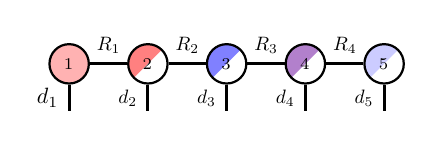
\begin{tikzpicture}[baseline=-0.5ex]
    \tikzset{tensor/.style = {minimum size = 0.5cm,shape = circle,thick,draw=black,inner sep = 0pt}, edge/.style = {thick,line width=.4mm},every loop/.style={}}
    \def\x{0}
    \def\y{0}
    \node[tensor, 
        fill=red!30!white, shift = {(\x-4,\y)}] (A) {\scalebox{0.85}{$\At_1$}};
        \draw[edge](A) -- (\x-4,\y-0.6) node [midway,left] {\scalebox{0.8}{\dimcolor{$d_1$}}};
       \node[tensor, path picture={
        \fill[fill=red!50!white](path picture bounding box.south west)
        -- 
        (path picture bounding box.north east) --
        (path picture bounding box.north west) -- cycle;
        }, shift={(\x-3,\y)}] (B) {\scalebox{0.85}{$\At_2$}};
       \draw[edge](B) -- (\x-3,\y-0.6)node [midway,left] {\scalebox{0.7}{\dimcolor{$d_2$}}};
        \node[tensor, path picture={
        \fill[fill=blue!50!white](path picture bounding box.south west)
        -- 
        (path picture bounding box.north east) --
        (path picture bounding box.north west) -- cycle;
        }, shift={(\x-2,\y)}] (C) {\scalebox{0.85}{$\At_3$}};
        \draw[edge](C) -- (\x-2,\y-0.6)node [midway,left] {\scalebox{0.7}{\dimcolor{$d_3$}}};
        \node[tensor, path picture={
       \fill[fill=blue!60!red!50!](path             picture bounding box.south west)
        -- 
        (path picture bounding box.north east) --
       (path picture bounding box.north west) -- cycle;}, shift={(\x-1,\y)}] (D) {\scalebox{0.85}{$\At_4$}};
    \draw[edge](D) -- (\x-1,\y-0.6)node [midway,left] {\scalebox{0.7}{\dimcolor{$d_4$}}};
    \node[tensor, path picture={
    \fill[fill= blue!20!white](path             picture bounding box.south west)
    -- 
    (path picture bounding box.north east) --
    (path picture bounding box.north west) -- cycle;}, shift={(\x,\y)}] (E) {\scalebox{0.85}{$\At_5$}};
    \draw[edge](E) -- (\x,\y-0.6)node [midway,left] {\scalebox{0.7}{\dimcolor{$d_5$}}};
    \draw[edge](A) -- (B) node [midway,above] {\scalebox{0.7}{\dimcolor{$R_1$}}};
    \draw[edge](B) -- (C) node [midway,above] {\scalebox{0.7}{\dimcolor{$R_2$}}};
    \draw[edge](C) -- (D) node [midway,above] {\scalebox{0.7}{\dimcolor{$R_3$}}};
    \draw[edge](D) -- (E) node [midway,above] {\scalebox{0.7}{\dimcolor{$R_4$}}};
\end{tikzpicture}~~~\text{step:~1}\\
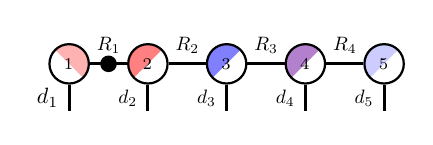
\begin{tikzpicture}[baseline=-0.5ex]
    \tikzset{tensor/.style = {minimum size = 0.5cm,shape = circle,thick,draw=black,inner sep = 0pt}, edge/.style = {thick,line width=.4mm},every loop/.style={}}
    \def\x{0}
    \def\y{0}
    \node[tensor, path picture = {
        \fill[fill=red!30!white] (path picture bounding box.south east)
        -- 
        (path picture bounding box.north west) --
        (path picture bounding box.north east) -- cycle;
        }, shift = {(\x-4,\y)}] (A) {\scalebox{0.85}{$\At_1$}};
        \draw[edge](A) -- (\x-4,\y-0.6) node [midway,left] {\scalebox{0.8}{\dimcolor{$d_1$}}};
         \draw  node[fill = black,circle,inner sep=0pt,minimum size=6pt] (m) at (\x-3.5,\y) {};
       \node[tensor, path picture={
        \fill[fill=red!50!white](path picture bounding box.south west)
        -- 
        (path picture bounding box.north east) --
        (path picture bounding box.north west) -- cycle;
        }, shift={(\x-3,\y)}] (B) {\scalebox{0.85}{$\At_2$}};
       \draw[edge](B) -- (\x-3,\y-0.6)node [midway,left] {\scalebox{0.7}{\dimcolor{$d_2$}}};
        \node[tensor, path picture={
        \fill[fill=blue!50!white](path picture bounding box.south west)
        -- 
        (path picture bounding box.north east) --
        (path picture bounding box.north west) -- cycle;
        }, shift={(\x-2,\y)}] (C) {\scalebox{0.85}{$\At_3$}};
        \draw[edge](C) -- (\x-2,\y-0.6)node [midway,left] {\scalebox{0.7}{\dimcolor{$d_3$}}};
        \node[tensor, path picture={
       \fill[fill=blue!60!red!50!](path             picture bounding box.south west)
        -- 
        (path picture bounding box.north east) --
       (path picture bounding box.north west) -- cycle;}, shift={(\x-1,\y)}] (D) {\scalebox{0.85}{$\At_4$}};
    \draw[edge](D) -- (\x-1,\y-0.6)node [midway,left] {\scalebox{0.7}{\dimcolor{$d_4$}}};
    \node[tensor, path picture={
    \fill[fill= blue!20!white](path             picture bounding box.south west)
    -- 
    (path picture bounding box.north east) --
    (path picture bounding box.north west) -- cycle;}, shift={(\x,\y)}] (E) {\scalebox{0.85}{$\At_5$}};
    \draw[edge](E) -- (\x,\y-0.6)node [midway,left] {\scalebox{0.7}{\dimcolor{$d_5$}}};
    \draw[edge](A) -- (B) node [midway,above] {\scalebox{0.7}{\dimcolor{$R_1$}}};
    \draw[edge](B) -- (C) node [midway,above] {\scalebox{0.7}{\dimcolor{$R_2$}}};
    \draw[edge](C) -- (D) node [midway,above] {\scalebox{0.7}{\dimcolor{$R_3$}}};
    \draw[edge](D) -- (E) node [midway,above] {\scalebox{0.7}{\dimcolor{$R_4$}}};
\end{tikzpicture}~~~~~~\text{QR}\\
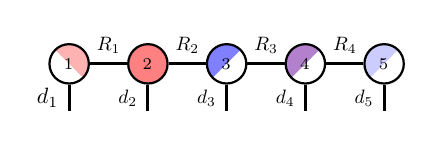
\begin{tikzpicture}[baseline=-0.5ex]
    \tikzset{tensor/.style = {minimum size = 0.5cm,shape = circle,thick,draw=black,inner sep = 0pt}, edge/.style = {thick,line width=.4mm},every loop/.style={}}
    \def\x{0}
    \def\y{0}
    \node[tensor, path picture = {
        \fill[fill=red!30!white] (path picture bounding box.south east)
        -- 
        (path picture bounding box.north west) --
        (path picture bounding box.north east) -- cycle;
        }, shift = {(\x-4,\y)}] (A) {\scalebox{0.85}{$\At_1$}};
        \draw[edge](A) -- (\x-4,\y-0.6) node [midway,left] {\scalebox{0.8}{\dimcolor{$d_1$}}};
       \node[tensor, 
        fill=red!50!white, shift = {(\x-3,\y)}] (B) {\scalebox{0.85}{$\At_2$}};
       \draw[edge](B) -- (\x-3,\y-0.6)node [midway,left] {\scalebox{0.7}{\dimcolor{$d_2$}}};
        \node[tensor, path picture={
        \fill[fill=blue!50!white](path picture bounding box.south west)
        -- 
        (path picture bounding box.north east) --
        (path picture bounding box.north west) -- cycle;
        }, shift={(\x-2,\y)}] (C) {\scalebox{0.85}{$\At_3$}};
        \draw[edge](C) -- (\x-2,\y-0.6)node [midway,left] {\scalebox{0.7}{\dimcolor{$d_3$}}};
        \node[tensor, path picture={
       \fill[fill=blue!60!red!50!](path             picture bounding box.south west) -- (path picture bounding box.north east) -- (path picture bounding box.north west) -- cycle;}, shift={(\x-1,\y)}] (D) {\scalebox{0.85}{$\At_4$}};
    \draw[edge](D) -- (\x-1,\y-0.6)node [midway,left] {\scalebox{0.7}{\dimcolor{$d_4$}}};
    \node[tensor, path picture={
    \fill[fill= blue!20!white](path picture bounding box.south west)
    -- 
    (path picture bounding box.north east) --
    (path picture bounding box.north west) -- cycle;}, shift={(\x,\y)}] (E) {\scalebox{0.85}{$\At_5$}};
    \draw[edge](E) -- (\x,\y-0.6)node [midway,left] {\scalebox{0.7}{\dimcolor{$d_5$}}};
    \draw[edge](A) -- (B) node [midway,above] {\scalebox{0.7}{\dimcolor{$R_1$}}};
    \draw[edge](B) -- (C) node [midway,above] {\scalebox{0.7}{\dimcolor{$R_2$}}};
    \draw[edge](C) -- (D) node [midway,above] {\scalebox{0.7}{\dimcolor{$R_3$}}};
    \draw[edge](D) -- (E) node [midway,above] {\scalebox{0.7}{\dimcolor{$R_4$}}};
\end{tikzpicture}~~~\text{step:~2}\\
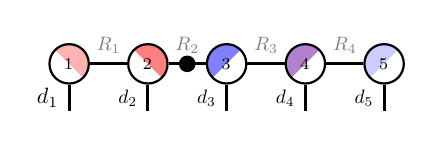
\begin{tikzpicture}[baseline=-0.5ex]
    \tikzset{tensor/.style = {minimum size = 0.5cm,shape = circle,thick,draw=black,inner sep = 0pt}, edge/.style = {thick,line width=.4mm},every loop/.style={}}
    \def\x{0}
    \def\y{0}
    \node[tensor, path picture = {
        \fill[fill=red!30!white] (path picture bounding box.south east)
        -- 
        (path picture bounding box.north west) --
        (path picture bounding box.north east) -- cycle;
        }, shift = {(\x-4,\y)}] (A) {\scalebox{0.85}{$\At_1$}};
        \draw[edge](A) -- (\x-4,\y-0.6) node [midway,left] {\scalebox{0.8}{\dimcolor{$d_1$}}};
       \node[tensor, path picture={
        \fill[fill=red!50!white](path picture bounding box.south east)
        -- 
        (path picture bounding box.north west) --
        (path picture bounding box.north east) -- cycle;
        }, shift={(\x-3,\y)}] (B) {\scalebox{0.85}{$\At_2$}};
       \draw[edge](B) -- (\x-3,\y-0.6)node [midway,left] {\scalebox{0.7}{\dimcolor{$d_2$}}};
        \draw  node[fill = black,circle,inner sep=0pt,minimum size=6pt] (m) at (\x-2.5,\y) {};
        \node[tensor, path picture={
        \fill[fill=blue!50!white](path picture bounding box.south west)
        -- 
        (path picture bounding box.north east) --
        (path picture bounding box.north west) -- cycle;
        }, shift={(\x-2,\y)}] (C) {\scalebox{0.85}{$\At_3$}};
        \draw[edge](C) -- (\x-2,\y-0.6)node [midway,left] {\scalebox{0.7}{\dimcolor{$d_3$}}};
        \node[tensor, path picture={
       \fill[fill=blue!60!red!50!](path             picture bounding box.south west)
        -- 
        (path picture bounding box.north east) --
       (path picture bounding box.north west) -- cycle;}, shift={(\x-1,\y)}] (D) {\scalebox{0.85}{$\At_4$}};
    \draw[edge](D) -- (\x-1,\y-0.6)node [midway,left] {\scalebox{0.7}{\dimcolor{$d_4$}}};
    \node[tensor, path picture={
    \fill[fill= blue!20!white](path             picture bounding box.south west)
    -- 
    (path picture bounding box.north east) --
    (path picture bounding box.north west) -- cycle;}, shift={(\x,\y)}] (E) {\scalebox{0.85}{$\At_5$}};
    \draw[edge](E) -- (\x,\y-0.6)node [midway,left] {\scalebox{0.7}{\dimcolor{$d_5$}}};
    \draw[edge](A) -- (B) node [midway,above] {\scalebox{0.7}{\textcolor{gray}{$R_1$}}};
    \draw[edge](B) -- (C) node [midway,above] {\scalebox{0.7}{\textcolor{gray}{$R_2$}}};
    \draw[edge](C) -- (D) node [midway,above] {\scalebox{0.7}{\textcolor{gray}{$R_3$}}};
    \draw[edge](D) -- (E) node [midway,above] {\scalebox{0.7}{\textcolor{gray}{$R_4$}}};
\end{tikzpicture}~~~~~~\text{QR}\\
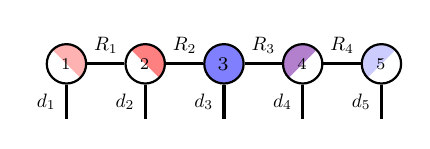
\begin{tikzpicture}[baseline=-0.5ex]
    \tikzset{tensor/.style = {minimum size = 0.5cm,shape = circle,thick,draw=black,inner sep = 0pt}, edge/.style = {thick,line width=.4mm},every loop/.style={}}
    \def\x{0}
    \def\y{0}
 \node[tensor, path picture={
        \fill[fill=red!30!white](path picture bounding box.south east)
        -- 
        (path picture bounding box.north west) --
        (path picture bounding box.north east) -- cycle;
        }, shift={(\x,\y)}] (A) {\scalebox{0.85}{$\At_1$}};
        \draw[edge](A) -- (\x,\y-0.7) node [midway,left] {\scalebox{0.7}{\dimcolor{$d_1$}}};
       \node[tensor, path picture={
        \fill[fill=red!50!white](path picture bounding box.south east)
        -- 
        (path picture bounding box.north west) --
        (path picture bounding box.north east) -- cycle;
        }, shift={(\x+1,\y)}] (B) {\scalebox{0.85}{$\At_2$}};
         \draw[edge](B) -- (\x+1,\y-0.7)node [midway,left] {\scalebox{0.7}{\dimcolor{$d_2$}}};
         \node[tensor,fill=blue!50!white] (C) at (\x+2,\y){$\At_3$};
          \draw[edge](C) -- (\x+2,\y-0.7)node [midway,left] {\scalebox{0.7}{\dimcolor{$d_3$}}};
          \node[tensor, path picture={
        \fill[fill=blue!60!red!50!](path picture bounding box.south west)
        -- 
        (path picture bounding box.north east) --
        (path picture bounding box.north west) -- cycle;
        }, shift={(\x+3,\y)}] (D) {\scalebox{0.85}{$\At_4$}};
         \draw[edge](D) -- (\x+3,\y-0.7)node [midway,left] {\scalebox{0.7}{\dimcolor{$d_4$}}};
        \node[tensor, path picture={
        \fill[fill=blue!20!white](path picture bounding box.south west)
        -- 
        (path picture bounding box.north east) --
        (path picture bounding box.north west) -- cycle;
        }, shift={(\x+4,\y)}] (E) {\scalebox{0.85}{$\At_5$}};
         \draw[edge](E) -- (\x+4,\y-0.7)node [midway,left] {\scalebox{0.7}{\dimcolor{$d_5$}}};
    \draw[edge](A) -- (B) node [midway,above] {\scalebox{0.7}{\dimcolor{$R_1$}}};
    \draw[edge](B) -- (C) node [midway,above] {\scalebox{0.7}{\dimcolor{$R_2$}}};
    \draw[edge](C) -- (D) node [midway,above] {\scalebox{0.7}{\dimcolor{$R_3$}}};
    \draw[edge](D) -- (E) node [midway,above] {\scalebox{0.7}{\dimcolor{$R_4$}}};
\end{tikzpicture}~~~\text{step:~3}
\caption{TT-ALS 的一次半扫描}\label{fig:ortho-tt-als-alg}
\end{figure}
图~\ref{fig:ortho-tt-als-alg} 给出了 TT-ALS 的一次半扫描。在每一个非 QR 步骤中，完全着色的核心张量被优化；在每一个 QR 步骤中，非正交分量（用黑色圆圈表示）~被吸收进下一个核心张量。这一过程不断重复直到抵达分解的右端，然后再从右端重复同样的过程直到抵达左端（图中未展示）。整个过程反复进行直至收敛。 
\begin{remark}
    除重构误差之外，该算法还可配合其他损失函数使用。此时，损失关于某个核心张量的优化未必归结为最小二乘问题，因而不再称为 ALS，而只是 \emph{交替最小化}。该算法还有一个双站点变体：在每次迭代中，把相邻的两个核心张量合并后联合优化，再用截断奇异值分解将其重新一分为二~\citep{holtz2012alternating}。
\end{remark}

